\documentclass[11pt]{pnas-new}
% \documentclass[10pt]{article}
\templatetype{pnasresearcharticle} % Choose template 
% {pnasresearcharticle} = Template for a two-column research article
% {pnasmathematics} %= Template for a one-column mathematics article
% {pnasinvited} %= Template for a PNAS invited submission

\usepackage[utf8]{inputenc}
\usepackage[T1]{fontenc}
\usepackage{xcolor,ulem}
\usepackage{mdframed}
\usepackage{wrapfig}
\usepackage{multicol}
\setlength{\columnsep}{1cm}
\usepackage{graphicx}
\usepackage{adjustbox}
\usepackage{lipsum}
\newlength{\strutheight}
\usepackage{soul} % for strike-through (\st)



\author[1]{Yoav Freund}
\author[2]{Hau-Tieng Wu}
\affil[1]{UCSD, Computer Science, San Diego, 92093, United States}
\affil[2]{Duke, Mathematics and Statistical Science, Durham, 27708, USA}

\title{You should prefer a digital Doctor that can say\\ "I don't know"}

\newcommand{\comment}[3]{{\color{#1} {\bf #2 :} #3}}
%\newcommand{\comment}[3]{}  % suppress comments
\newcommand{\hautieng}[1]{\comment{blue}{Hautieng}{#1}}
\newcommand{\yoav}[1]{\comment{red}{Yoav}{#1}}

\mdfsetup{middlelinecolor=blue, middlelinewidth=2pt, backgroundcolor=blue!10, roundcorner=10pt}

\mdfdefinestyle{Medicine}{middlelinecolor=red, middlelinewidth=2pt, backgroundcolor=red!10, roundcorner=10pt}
\mdfdefinestyle{ML}{middlelinecolor=green, middlelinewidth=2pt, backgroundcolor=green!10, roundcorner=10pt}
\mdfdefinestyle{Org}{middlelinecolor=blue, middlelinewidth=2pt, backgroundcolor=blue!10, roundcorner=10pt}

\newcommand{\block}[3]{
  \begin{wrapfigure}{r}[34pt]{-10pt}
    \begin{minipage}[t]{12cm}
      \begin{mdframed}[style=#1]{\footnotesize{\bf #2}\\ #3} \end{mdframed}
    \end{minipage}
  \end{wrapfigure}
}
\newcommand{\Medicine}[2]{\block{Medicine}{#1}{#2}}
\newcommand{\ML}[2]{\block{ML}{#1}{#2}}
\newcommand{\Org}[2]{\block{Org}{#1}{#2}}



\begin{abstract}

  The meteoric rise of AI in general and Deep Learning in particular
  is generating great excitement throughout academia and commerce, and
  in particular in medicine\cite{topol2019deep,
    wachter2015digital}. With some some high-profile claims~\cite{}
  that AI will soon replace humans in many medical specialties.

  In this position paper we present an alternative view. We contrast
  {\em Artificial Intelligence} with {\em Intelligence Augmentation}
  and argue that the second is more likely to benefit the patient than
  the first. We provide evidence to this argument and present a vision
  in which easier decisions are delegated to computers, while the more
  difficult ones are handled by humans.

\end{abstract}

\begin{document}
\settoheight{\strutheight}{\strut}

 
\maketitle

%\thispagestyle{firststyle}

The meteoric rise of AI and Deep learning raises the possibility that
doctors will be replaced computers~\cite{Mukherjee2017}. Geoff Hinton,
a famous deep learning researcher said in 2017: ``It's just completely
obvious that in ten years deep learning is going to do better than
Radiologists ... They should stop training radiologists now''.

The predictions of Sebastian
Thrun~\cite{Mukherjee2017,esteva2017dermatologist}, another leader in
machine learning, are less disruptive: ``... deep learning devices
will not replace dermatologists and radiologists. They will {\em
  augment} professionals, offering the expertise and assistance''. In
this article we argue for Thrun's prediction and explain why
augmentation, rather than replacement, is the approach more likely to
prevail.

\Org{Artificial Intelligence and Intelligence Augmentation}{
The driving question of AI can be summarized as: ``are machines
  capable of behaving in a way that indistinguishable from that of
  humans, as judged by other humans''.  The archetypal test
  of whether artificial intelligence has been achieved is the {\em Turing
  Test}, in which a human, communicating with another agent through
  text alone, is unable to tell whether or not the agent is human. A
  natural consequence of computers being indistinguishable from humans
  is that they will be replacing humans, causing mass unemployment.

  The driving question of IA is whether and how computers can be used 
to {\em augment} humans rather than replace them. Some augmentations
are the territory of science fiction. For example,
cyborgs whose anatomy is part human, part artificial and can with
equal ease solve complex equations or write poetry. Other examples are
so mundane that they are taken for granted. Examples
are the smart phone and google search, with which our capabilities are augmented by computers. 
 
The Turing test was published~\cite{turing1951can} in 1951. A 1956
workshop in Dartmouth college is widely recognized as the beginning of
the field of AI. IA appeared on the scene around the same time, with
Ashby~\cite{ashby1956introduction} in 1956
Licklider~\cite{licklider1960man} in 1960 and
Englbart~\cite{engelbart1962augmenting} in 1962.

Arguably, the impact of IA on today's society is much larger than
that of AI. Siri, Google search and assisted driving are some of the
common apps that augment human ability. On the other hand, the goal of
creating a general purpose AI that possesses a human-like capability
to reason about new domains seems to be as far as ever.  At the same
time, AI holds the fascination of many, possibly because of its
tantalizing combination of promise and threat.}

 The question of whether dermatologists will be
replaced by computers or be empowered by computers is but a recent
incarnation of a debate between AI (Artificial Intelligence) and IA
(Intelligence amplification) which has a long history (see inset). To
distinguish between AI and IA we use the terms ``AI agent'' vs. ``IA
sidekick''. This terminology contrasts {\em agents}, which are endowed
with {\em agency} and can take {\em actions} that effect the patient's
health, with {\em sidekicks} which can provide advice and suggestions,
but who are not allowed to take action.

Replacing dermatologists with AI agents can bring cost savings,
but is likely to lead to inferior care. One of the reasons is that it
is hard for AI to make a human connection with the patient and thereby
take into consideration personal, social, financial and mental factors.

On the other hand, IA powered sidekicks IA can help the medical staff
detect and diagnose medical problems quickly, efficiently,
accurately. This can lead to cost savings, especially for homebound
patients suffering from chronic diseases.

Central to our approach is a quantification of {\em prediction
  confidence}. Such quantification is needed to avoid premature
diagnostic conclusions, and to decide which additional tests or
consultations might be needed. Consider a doctor that is asked asked
to diagnose a patient with complex or conflicting symptoms. A careful
doctor will admit their uncertainty and perform additional tests or
ask a specialist. A less careful, overly self confident doctor is
likely give an incorrect diagnosis and choose an ineffective or even damaging
treatment plan.

An AI agent, trained to be better than the human doctor, might end up
behaving like an overly confident doctor. An IA sidekick, aware of
it's own limitations, will give advice only when the evidence is
strong and otherwise say ``I don't know''.

In the following sections we explore these ideas in more detail. We
start with a critique of one of the papers that claims that AI agents
can outpeform human diagnosticians.

\section{Supervised Learning and the Ground Truth}
\label{sec:ground-truth}

Deep learning is a special case of {\em supervised learning} (see
inset), sometimes called {\em input-output}
learning~\cite{ng2016artificial,topol2019deep}.
\ML{Supervised Learning and ground truth}{Roughly speaking, machine
  learning (ML) can be divided into {\em unsupervised} learning and
  {\em supervised} learning. In both cases, the task of the learning
  algorithm is transforming a set of {\em examples} into a {\em model}. In
  unsupervised learning, the examples are undifferentiated raw
  measurements. In supervised learning, which is the focus of
  this article, each example consists of an {\em input} and a {\em
    label}. Typically, the labels are provided by human
  experts. These labels {\color{red}are usually viewed as}\sout{define} the {\em ground truth} and the goal of
  the learning algorithm is to make predictions that diverge as little
  as possible from the ground truth.}


The data for supervised learning consists of a large collection
(input,output) pairs. For medical diagnosis, the inputs is medical
information for the patient (Heart rate, blood tests, X-ray images
etc.) and the output is the diagnosis. This output is considered the
``ground-truth'' and is assumed to represent the undisputed truth.

Here lies the the first difficulty with applying supervised learning
to medical diagnosis. In most real-world scenarios the diagnosis
does is not an objectively measurable fact, rather, it
represents the conclusion drawn by a fallible human diagnostician. We  will
return to this issue in the next section.

The other important assumption made in supervised learning is that the
generated classifier is tested using the same distribution of examples
as that of the training set.

We now consider a study in deep neural networks which claims to show
that DNNs can perform diagnostics as well as, or better, than human diagnosticians. 
\ML{Skin cancer diagnosis using Deep Neural Networks}{One of the
  papers that provided evidence that deep neural networks might be
  able to outperform humans is the work of Esteva et
  al~\cite{esteva2017dermatologist}. They trained a Deep neural
  network to classify images of skin into three categories: benign,
  malignant and non-cancerous. The network was then tested, along with
  twenty five dermatologists on images which were labeled by a
  pathologist analysis of the biopsy. The neural network performed
  comparably to, and sometimes better than the human dermatologist.
  To provide ground truth, the patients were biopsied and the piopsies
  were diagnosed by pathologists.
}  

In a highly cited paper in the journal
Science~\cite{esteva2017dermatologist} provides evidence supporting
the claim that computers can diagnose skin cancer as well or better than board
certified dermatologists.

A fundamental problem with the experiment is in the way the data was
collected. The data used in the experiment was {\em retrospective},
i.e. it was collected from the records of past patients for which both
a skin image and a biopsy were available. Normally, patients get
biopsied only if the dermatologist thinks there is a significant
chance of {\bf malignancy}. As a result, a retrospective study that is
based on patients for whom a biopsy was taken is likely to
over-represent malignant patients and therefor be biased. If an image-based classifier
is trained on the biased data, its performance on unbiased test data
is likely to be worse. Specifically, when the classifier is applied to skin
images of undiagnosed patients it is likely to over-diagnose them as
malignant. The practical implication would be that more patients than
necessary will be biopsied.

As we elaborate on in the next section, in medical diagnostics the
ground truth is usually not available, all that we have to go on are
the opinions of human diagnosticians.

\section{Uncertainty in medicine}

For the most part, it is hard to associate ground truth with medical
diagnostics. This is evident studies of {\em inter-rater agreement} (see
inset). In studies of this kind multiple doctors produce diagnostics
based identical medical information without communicating with each other. \input{Arrhythmia}

\Medicine{Inter-rater agreement}{A common method for measuring the
  level of agreement is an {\em inter-rater agreement studies}. In
  such studies several doctors are provided with the same patient
  file and are asked to give a diagnosis.

  A common measure of of the agreement between two raters is the Cohen's kappa
  coefficient, usually denoted by $\kappa$.  Kappa is computed from two more basic quantities: $0\leq a\leq 1$
  is the fraction of patient files on which the two raters agree, 
  and $0\leq c\leq 1$ is the fraction of agreements that would occur
  by chance. The definition of kappa is $\kappa=\frac{a-c}{1-c}$.

  If $\kappa=1$ The raters always agree, if $\kappa=0$ the rate of
  agreement corresponds to chance, and if $\kappa<0$ then the rate of
  agreement is lower than chance, i.e. the two raters tend to have
  different opinion. An
    interpretation of $\kappa$ recommended by Cohen
    \cite{mchugh2012interrater} is: $\kappa\leq 0$: no agreement, $0< \kappa\leq 0.20$:none to slight
    agreement, $0.2<\kappa\leq 0.40$: fair agreement,
    $0.4<\kappa\leq 0.60$ as moderate agreement, $0.6<\kappa\leq
    0.80$: substantial agreement, and $0.8<\kappa\leq 1.00$: perfect
    agreement.

    For example, in the sleep stage annotation, the pairwise Cohen's kappa over 5 sleep experts (totally 10 pairs) is on average 65\% over normal subjects and about 59\% over subjects with sleep apnea \cite{norman2000interobserver}. In other words, the inter-rater agreement is substantial over normal subjects and moderate over subjects with sleep apnea.
    %\yoav{can we give a list of kappa values for some common      diagnostics here?}
  }


In addition, diagnosis is not an input-output mapping. Rather, it
is an iterative process which reduces uncertainty over time. To
illustrate this, consider the diagnostics of a patient that is treated
in an out-patient clinique..  When a patient arrives at a clinique for
the first time, all diagnostics are possible. After a physical exam
and an interview with a doctor, , many possibilities are
eliminated. In {\em simple} cases, this is enough for the doctor to
confidently choose a treatment. In more complex cases, the doctor
might ask for multiple tests and visits, refer the patient to a
specialist, consult colleagues, journals and books etc. To choose a
treatment plan, the set of possible diagnostics has to be reduced
however, it does not have to be reduced to a {\em single} diagnostics,
as multiple diagnostics might share a treatment plan.

In order to apply a supervised learning method, such as  DNN, to the
diagnostic problem, we need to define a ground-truth label for each
patient. But that is easier said than done. As the final output of the
diagnostic process is a treatment plan, we would like to know what is
the best treatment plan. Unfortunately, we can only use a single
treatment plan to treat the patient, so the most that we might be able
to infer is whether the chosen treatment was effective.  Even if the
patient improved, the cause might have been unrelated to the
treatment. It might be due to a change in diet or reduction in stress.
Moreover, in most cases, there are few or none followup visits and as
a result there is no data as to whether the patient has a lasting
improvement in health.

We suggest a different goal for automatic diagnosis.
Rather than predicting the {\em ``correct''}
diagnosis we define the goal of the computer to be predicting the {\em
  distribution} of diagnosis across doctors. In addition, we allow
doctors to be uncertain of their own diagnosis.
The distribution of doctors predictions represents their confidence as
a group. In other words, by predicting that all doctors will agree on
the diagnosis, we assign high confidence to that diagnosis. 
If, on the other hand, we
predict that doctors will give one (or both) of two diagnoses A and B, then
our prediction is akin to saying ``we are confident that the prediction
is either A or B, to know which one we will need additional
tests''. This accurately represents our current state in the
diagnostic process and is more useful than deciding on one diagnostic
with insufficient evidence.


\iffalse
It is certainly expected that physicians can achieve a reliable
decision making, probably with sufficient clinical information
\cite{mehta2011agreement} or if only the major information is needed
\cite{atiya2003interobserver}. However, in many cases, the quality of
decision making might be jeopardized due to various reasons, among
which the uncertainty in medicine is non-negligible.
\yoav{I find the previous paragraph unclear and confusing, We should
  talk about it}
\fi

%Medical uncertainty as manifest by low inter-rater agreement consequence,
%can be found in many clinical problems
There are many causes for uncertainty in medical diagnosis. We briefly
describe four categories of problems: {\em signal quality}, {\em knowledge gap}, the limitations of {\em
  diagnostic protocols} and {\em alarm fatigue}.


By {\bf Signal Quality} we refer to the quality of the raw data
collected for medical diagnosis. Some diagnostic measures, such
as heart rate, blood pressure and temperature can be measured reliably
and accurately. On the other hand, modern
devices such as EKG, EEG, camera images, X-ray, ultra-sound and EMR
produce vast and highly variable data. The quality of this data
depends on may factors among them, the quality of the instruments, the
consistency of the human operator, the build of the patient etc.
\Medicine{Uncertainty due to signal quality}{Medical devices use a
variety of bio-sensors that measure record and analyze different
biometric signals. These signals vary in velocity, ranging from
low-velocity vital signs such as heart rate, oxygen saturation,
temperature and blood pressure, through high-velocity waveforms such
as ECG and EEG and medical imaging such as CT, X-ray, MRI and scanning
microscopes. Some signals, such as blood pressure or heart rate, can
be directly used in diagnosis.  Some other signals have to be
interpreted before they can be used in diagnosis. We use the acronym
HS (High Speed) to refer to those signals that require interpretation.

Interpreting HS is a significant fraction of the work of most
doctors. In addition, There are medical specialties such as
Radiology and Pathology that are devoted to interpreting HS. These
so-called ``Pattern Doctors'' are predicted to be the early adopters
of AI~\cite{topol2019deep} or IA.
HS provides critical detailed information about the patient's
health. However, the richness of the signal can make it susceptible to
nuisance variability from noise, limited resolution, operator error,
etc. The number of nuisance variables is very large and confounding. In the next
paragraph we give an example of one nuisance variable: the placement
of ECG leads on the patient's body.
  
For ECG signals to be correctly and consistently interpreted, it is
important that the leads are placed correctly on the patient's
body. Several standards for placement have been published, for example, the standard 12 leads ECG system
\cite{goldberger2017clinical}, the EASI system \cite{Dower1988}, and the Frank lead system \cite{frank1956accurate}. 
It is not always possible to achieve a consistent and precise sensor
placement for biomedical signal collection due to various reasons, for example, the torso variation caused by gender, age and living styles.
This uncertainty might be tolerable for some clinical applications;
for example, an imprecise ECG sensor placement might not impact the
identification of some types of arrhythmia from the ECG signal, like
atrial fibrillation. However, this uncertainty might cause troubles in
identifying other types of arrhythmia, for example, premature atrial contraction.

}


Knowledge gap bla bla
   \Medicine{Knowledge gap}{ 
  Medical science is constantly evolving. This means
  that at any point of time, some medical facts are outside the
  collective knowledge of the medical profession. We refer to this as
  the {\em knowledge gap}.
  
  As the writing of this article, {\em COVID-19} is a worldwide crisis
  \cite{sohrabi2020world}. Back in Jan 2020, when it was first
  reported in China, very little was known about the disease or how to
  treat it.  Knowledge was quickly accumulated during the last 
  months. For example, we know more about hydroxychloroquine,
  remdesivir, and other candidate
  drugs~\cite{sanders2020pharmacologic,goldman2020remdesivir} and some
  treatment protocols have been
  developed~\cite{world2020population,world2020protocol,nakajima2020covid,awad2020perioperative}.
  Still, much is still unknown about COVID-19.
  
Knowledge gaps not only exist in new diseases, but
also exist in some well known maladies that have been studied for a
long time.
For example, Urodynamics, whose aim is to understand the movement of urine
through the bladder, sphincters, and urethra has been studied since
the 1800's~\cite{perez1992history}.
Urodynamic studies provide reliable time series of the pressure
dynamics in the bladder and sphincter. These time series are used
by urologists to decide how to treat patients at risk for
renal damage~\cite{abrams2003describing}, incontinence, frequent
urination, recurrent urinary tract infections, etc.
There are several well-established protocols for interpreting
detrusor pressure time
series.\cite{bauer2015international,austin2016standardization}.
When following these protocols, the urologist needs to identify
occurrences of an important short-term event called {\em detrusor
overactivity}.  However, as there is no precise definition of a detrusor
overactivity, the identification of these events is based 
on subjective judgements.  This has led to a significant inter-rater
disagreement in the analysis of detrusor pressure time series.
\cite{venhola2003interobserver,dudley2018interrater}.
}



\newpage
Another factor that impacts the accuracy and consistency of the
diagnosis is the uniformity of criteria across doctors and institutions
  \Medicine{Protocol limitation}{
  \sout{\yoav{For readers that are not MD, we should explain what are protocols, how they are generated, and whether all or some of their functionality ca be taken over by a computer. Also, I would put "extrapolation error" in here}}
  {\color{blue}According to NCI dictionaries, protocol means a detailed plan of a scientific or medical experiment, treatment, or procedure. \url{https://www.cancer.gov/publications/dictionaries/cancer-terms/def/protocol}. In clinics, it is a document that guides decision making, including criteria regarding diagnosis, management, and treatment. It exists in different areas of healthcare with different formats. In a loose sense, it could be understood as an algorithm solving a given mathematics problem. However, unlike the relationship between an algorithm and a mathematics problem, a medical protocol might not cover every situation and provide all possible solutions, and have several limitations.}
  
  
  The American Academy of Sleep
    Medicine (AASM) publishes criteria for manual sleep stage
    and
    sleep apnea annotation from the gold standard sleep study instrument, the polysomnogram (PSG). This annotation is based on manual analysis
    of biosignals recorded from the PSG \cite{Iber2007,berry2012aasm}. The AASM is a protocol that has been extensively applied, with rigorous scientific support, and updated regularly according to latest evidences. 
    %
    A detail sleep profile is critical for sleep quality enhancement, or even medical condition improvement.
    %
    However, it is well known that even with the well established protocol, the inter-rater agreement rate of sleep stage annotation among experienced experts, {\color{blue}in terms of percentage of epoch-by-epoch agreement, is only about 76\% over normal subjects and about 71\% over subjects with sleep apnea, while the Cohen's kappa is 65\% over normal subjects and about 59\% over subjects with sleep apnea}  \cite{norman2000interobserver}. Among many reasons, the one that is directly related to the intelligent system development is how the criteria are ``described'' in the protocol. For example, it is described in the protocol that if the delta wave occupies more than 20\% of a given 30-second epoch of the electroencephalogram during sleep, that 30-second epoch is defined to be the N3 stage. 20\% of a given 30-second epoch is 6 seconds. What about if the delta wave occupies 5.99-, or 6.01-seconds? What about if the delta wave sustains for 10 seconds, but it is divided into two consecutive 30-second epochs? When sitting on the ``gray area'' that is inherited from 
  the protocol, sleep experts need to make a
  decision based on their experience or the information
  they have at hand, and this leads to medical uncertainties, and hence the inter-rater, or even intra-rater disagreement.  
  
  {\color{blue}Another protocol limitation is the}
  ``extrapolation error''; that is, when we apply the developed
  protocol to the population different from the population that we
  collect the evidence for the protocol \cite{brosnan2015modest}. {\color{blue}Such extrapolation error usually comes from the variability among subjects. If such variability is big, it
  limits the development of a more quantitative protocol
  \cite{venhola2003interobserver}, and different protocols might be
  needed for different situations.}
}


\newpage
bla bla
\Medicine{Alarm fatigue}{ Patient monitors are bedside medical devices
  that monitor patients that are at risk but currently stable, freeing
  the medical staff to attend to the patients whose status is
  critical.  Unfortunately, Patient monitors suffer from signal
  quality issues and tend to generate false alarms at a high
  rate. Over time, this can result in the staff not responding to
  alarms, potentially resulting in great damage to the patient. This
  phenomenon, called {\em alarm fatigue} (or alarm overload) is a
  major problem in hospital care \cite{brief2019top}. See, for example,  \cite{cvach2012monitor,paine2016systematic}, for a review.
  
  \yoav{Two questions: (1) Which of these papers are about the severity of the problem and which are about research? {\color{blue}-- Updated.} (2) regarding research, has there been research aimed at making the monitors adaptive to the patient and or nurse? {\color{blue}-- to my knowledge, they are adaptive to patients. The focus is reducing the patients' risk by reducing the false alarm.}} 
  
  Alarm fatigue is a well known issue medical providers encounter when working with patient monitors. It is frequently named as a threat to patient safety \cite{sendelbach2013alarm,ruskin2015alarm}, and a lot of research has been carried out toward this problem based on different techniques; for example, signal quality control \cite{li2012signal,behar2013ecg} or superalarm \cite{bai2016sequence,hu2019algorithm}, to name but a few.
}



% {\color{blue}Besides the above-mentioned reasons, there are more. For
%   example,} in some situations, when the needed information is
% missing, it is challenging to make a differential diagnosis
% \cite{moncada2011reading}.  {\color{blue}Despite the variety of
%   reasons, the key message here is that medical uncertainty is a
%   non-negligible fact in medicine.}

%   A direct consequence of the low inter-rater agreement rate is that the trained intelligent system might be questionable.
   
It is clear that such intelligent system is questionable and might
raise concerns. Recently, various regulations in this regard have been
proposed \cite{price2014black,ford2016privacy}.


Now, suppose we are able to eliminate all challenges from data
calibration and validation issues, and we can provide as much
information as possible to train the intelligence system. Even under
this assumption, it is clear that the system still suffers from the
protocol limitation or knowledge gap issues. Can such system be useful
in clinics? To answer this question, we should not forget that
physicians also follow the same protocol and have knowledge
gaps. Depending on the clinical problems, and the experience of
physicians under consideration, the agreement rate varies. Usually,
intern doctors know the least, while a senior attending knows the
most. It is natural that we trust a senior expert more, but it does
not mean that we do not trust a junior intern doctor.

\section{How to augment doctors}
Medical diagnosis is often uncertain or inconclusive. On the other
hand, a doctor responsible for a patient's health has to make
decisions in spite of this uncertainty. If the uncertainty presents a
sufficiently small risk, the doctor can choose a treatment. Otherwise
the doctor might consult other doctors, a medical journal or a book. 

To better understand the process and the possible place of AI in it,
we turn to the Kahaneman's~\cite{kahneman2011thinking} ``Thinking Fast Thinking Slow'' and
to Vordermark book on medical decision
making~\cite{vordermark2019introduction}.

Medical diagnosis can be divided into two main types: {\em
  recognition} and {\em elimination}. Recognition is a fast mental
process that is partially unconscious where the one correct diagnosis presents itself in the doctors mind.  Sometimes the doctor is not able to explain their recognition in words, which hinders discussion and documentation.  As recognition 
typically points to a single diagnosis, there is a danger that the
recognized diagnosis will hide other possible diagnoses.
Elimination, on the other hand, is a slow deliberate process  which starts with all possible diagnoses and gradually eliminates
unlikely ones based on patient history, examination and test
results. As Elimination is deliberative, it is easier to discuss and
document it.

In both recognition and elimination, past experience plays an important role. This experience is based on medical practice as well as knowledge learned from lectures or books. 

IA can aid the doctor both in Recognition and in Elimination. On the Recognition side, an IA can sift through massive data and point the diagnostician to suspicious areas.

On the Elimination side, an IA system could help carefully and systematically
eliminate diagnoses. This can help the doctor stay aware of possibilities that are not obvious, for differential diagnosis.


\iffalse
To make a decision based
on elimination, slow thinking with focused attention is critical
\cite{michel2020thinking}. 

An intelligent system could be extremely helpful for this
purpose. An intelligent system could help carefully and slowly
eliminate possible choices, and if it end up in a gray zone with
multiple possibilities, it says IDK. This would dramatically help
physicians daily practice.


{\bf Sources of uncertainty in medical diagnosis.}
\begin{itemize}
  \item{\bf The diagnostic process of elimination}
  \item{\bf Data Quality, Calibration, resolution} Discuss issue as placement of sensors, .
  \end{itemize}

 {\bf Hiding Uncertainty}
  \begin{itemize}
    \item {\bf Psychological reasons} Both doctor and patient prefer
      the projection of certitude.
    \item {\bf Protocols} --done
    \item {\bf diagnostic devices} Secrecy of the internal code limits
      the trustworthiness of the alarms.--done
    \item{\bf Alarm Fatigue}--done
  \end{itemize}
\fi
%{\bf Psychological reasons} Both doctor and patient prefer

How to quantify IDK? We should discuss how to quantify the confidence, or certainty, a physician has when making a decision. 
\ML{Certainty and conditional probability}{
This certainty is very different from the the conditional probability of the disease given the diagnostic. The first is
      akin to saying: 95\% of the dermatologists would give the same
      diagnostics. The second defines the probability that, if we had
      access to ground truth, then 95\% of the patients that receive
      this diagnostics have the corresponding condition.
}  
Clearly, experience leads to confidence. With more experience aggregated, diagnostic options that contradict the accumulated
  experience are eliminated, and hence more problems that need to be handled by the elimination process can be handled by the recognition process. However, facing our complicated human body, it is almost not possible for any single physician to aggregate all necessary experience to be confident about anything, so IDK is still an option. A practical and simple way to increase diagnostic certainty is to solicit the experience of a diverse group of doctors via discussion. If there is a clear majority for one diagnostic outcome,
      then the overall confidence in that diagnostics is high. While this voting procedure might guarantee the optimal outcome, it eliminates the uncertainty during the whole procedure. With this certain procedure, even if the outcome is negative, it can be traced back and accumulate evidence and experience. 

\section{How to augment medical institutions}

  Computer {\color{blue}has been} an integral part of medical practice {\color{blue}for decades}. From
  {\color{blue}electronic} medical records (EMR) to medical instrumentation to billing,
  hospitals and cliniques cannot function without computers. By some
  measures computers can already make better diagnosis than human
  doctors. The question is not {\em whether} computer diagnostics will
  become part of medical practice, the question is {\em how}.

  Some claim that human doctors and nurses are heading to extinction,
  following the fate of manufacturing jobs and bank cashiers.  Our
  prediction is that computers will change the nature of medical
  work. Our prediction is that the adaptation of IA will increase,
  rather than decrease, the number of healthcare workers. especially
  in the care of chronic disease and aging \st{and exploring the
    nature of our complicated human body}.

  Consider an established clinique or hospital. While every day brings
  in new cases, it is likely that for many of these cases the
  diagnosis is ``easy'', i.e. the same diagnosis would be given by
  most doctors. If the IA sidekick identify a significant fraction of
  the patients that are clearly sick or the patients that are clearly
  ok, then it can help the staff prioratize treatment. For example,
  patients identified in critical condition can get to see a senior
  doctor faster, while patients that are confidently identified as
  healthy are directed to a junior doctor or to a nurse practitioner.

\yoav{Until here}
  
  
  We believe computers {\em can} perform accurate diagnosis for cases where
  different doctors are likely to agree. In other cases {\color{blue}that are in the}
  diagnostic gray area, the computer will output ``I don't know'' and
  transfer the responsibility to the doctor. In most cases, the doctor
  cannot say ``I don't know'' because she is responsible for the
  patients health. On the other hand, resolving the diagnostic
  question is not her only choice. She can consult another doctor or
  the literature, ask for additional tests, or decide on a treatment
  based on available information. Deciding between these options requires much
  more than diagnostic information. It involves understanding the
  patient's emotional, mental and financial state, the patient's
  support system, the strengths and weaknesses of the hospital in
  which this is taking place etc. {\color{blue}Such exploration and results will be fed back to the system to reduce the gray area, which is similar to training an intern doctor in the hospital.}

  Over time, computers will be able to take into consideration more
  and more of this complex information. However, for the foreseeable
  future, it is unlikely that computers will be given the
  responsibility to make medical {\em decisions}. Computers
  will take on much of the diagnostics and alarm tasks, improving the
  accuracy and timeliness of the doctors actions. Computers will
  output IDK in gray areas and will leave the decision making to the
  human doctor. Giving the computer the authority to make decisions
  currently done by human doctors will {\color{blue}not only} deprive the patient the human
  attention of the doctor{\color{blue}, but also put patients in risk}.

  Some of the digitization of the medicine has come between patients
  and doctors. {\color{blue}A common impression from the learning perspective is that physicians need to record more activities and hence reduce the amount of time on interacting with patients. However, we} %\sout{The need to record all activities into the EMR system requires doctors to spend more time at the keyboard, reducing the amount of time of physical examination an discussion}. \hautieng{I guess I know what you want to say, but to be safe, I'll do the edit here after we chat.} 
  believe that {\color{blue}a properly designed } IA {\color{blue}that knows IDK} can
  move medicine in the opposite direction, letting the computer make
  the common noncontroversial diagnostics and giving the patient more
  time to interact with the patient.

%\begin{figure}[h]
%\begin{center}
%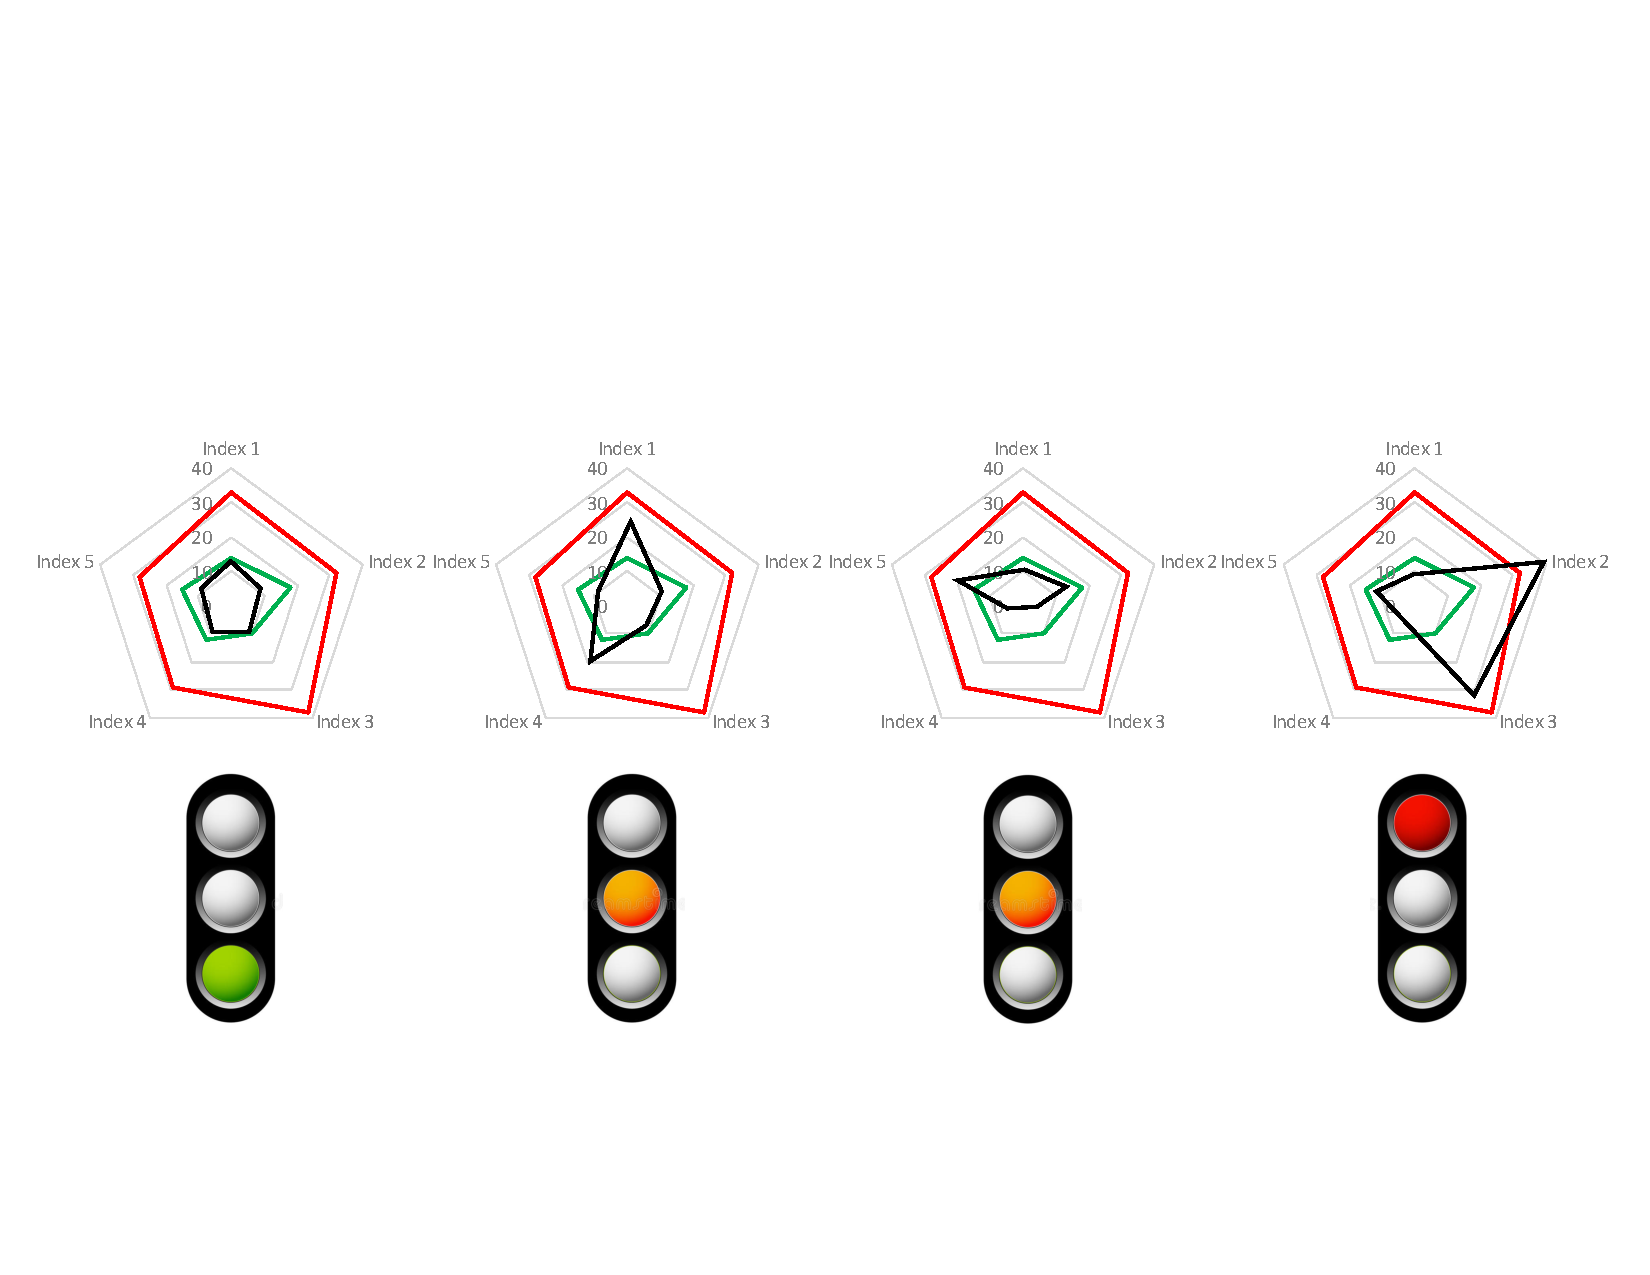
\includegraphics[trim=0 100 0 200,clip,width=7in]{figures/RedYellowGreen2.pdf}
%\caption{An illustration of how an alarm system works as a radar system. The red and green pentagons indicate the danger and safe region of five indices. A set of indices inside the green pentagon is safe (shown as a green light). If any index is outside the red pentagon, the patient is surely in danger (shown as a red light). However, if any index is outside the green pentagon but inside the red pentagon, the patient is in a ``gray zone'', or marginal situation, the system might not be able to decide the situation, and will report IDK (shown as a yellow light).\label{Figure IDK light}}
%\end{center}
%\end{figure}

  For IA technology to be widely adopted, the nurses and doctors that
  use them should experience an improvement in their practice {\color{blue}with the IA system. One example of such system is}
  that the display of the diagnostics computer uses a three color code
  to identify {\color{blue}the pre-defined status. In this system,} green indicates a confident
  negative diagnostic, red corresponds to a confident positive
  diagnosis, and yellow corresponds to IDK, meaning that the
  computer cannot confirm or reject the diagnostic outcome. {\color{blue}%See Figure \ref{Figure IDK light} for an illustration of such a system with a radar display. The thresholds that define these three ranges depend on our knowledge, and the data uncertainty and protocol issues should be taken into account. 
  With the IA system with IDK, healthcare providers could focus their time on patients overall situation, communication for life plan, or other interactions, and intervene the medical diagnostics when the IA system says IDK.}

%  The thresholds which define the three ranges .... \hautieng{discuss.}


  
  We finish this section with a few application areas which seem ready
  for applications of IA.
  
\begin{itemize}
\item{\bf Computer aided diagnostics for large-scale data}\\
  Medical imaging devices such at digital X-ray, CT, EMR and scanning
  microscope generate many gigabytes of data for each
  patient. Radiologists and pathologists spend their days analyzing
  these images to diagnose the patient. The large size and high
  resolution of the images on the one hand, and the time limitation on
  the analyst on the other imply that the analyst has to quickly
  narrow down the suspicious region, increase the chance of missing
  dangerous abnormalities.

  IA can help the pathologist by suggesting locations in the high
  resolution image that might contain cancer nodules~\cite{}.

  directing her attention to the
  parts of the image that are 

\item{\bf Adaptive Patient monitors}

{\color{blue} By further accumulating knowledge, reducing data uncertainty, and improving protocol, it is expected that the gray zone a well developed IA system has is small, and the alarm fatigue issue is alleviated since it only makes an alarm when it runs into IDK. There are many other aspects such an IA system equipped with IDK could help. Since the system knows IDK, it knows what is affirmative. When a medical decision made by a physician falls in the affirmative area, the IA system could help doubly confirm if the decision has any risk not considered by the physician. Such alarm, when sufficiently accurate, could help improve patient risk and healthcare quality. Eventually, this IA system could be evolved into a second opinion provider to healthcare providers. 
}


  
\item {\bf Dissemination of expertise}

Computers, trained by experts, can help novices. {\color{blue}A well-trained IA system equipped with IDK can provide confirmed answers to inexperienced physicians, and} serve a function
similar to score-cards{\color{blue}. Moreover, it can be applied to areas with scarce health resource. The system can provide local healthcare providers knowledge they do not know, and be connected back to physicians with richer medical knowledge when it runs into IDK.
On the high level, eventually, we can view an IA system with IDK as a medical specialist full of knowledge and do not make mistake when it knows the answer. When it encounters IDK, it will not hide it. The feedback from experienced physicians, or newly developed knowledge, could be input to decrease the gray areas, and reduce the chance of encountering IDK. Such system in the beginning behaves like an intern doctor, and teaching it is like}
teaching young diagnostics. {\color{blue}Due to the brain capacity and physical limitation, it is impossible for a single physician to know everything in every field, and it is possible that even a very experienced physician could make a mistake. Such a well trained IA system can eventually serve as a reliable second opinion provider to experienced physicians.}
\end{itemize}

\section{Summary}

%\bibliographystyle{alpha} 
\bibliography{medbib}

\end{document}